\begin{sloppypar}

\subsection{Fenster}

Die Klasse \texttt{czg.MainWindow} stellt das Spielfenster
dar und beinhaltet die \texttt{main}-Methode sowie eine
Reihe von statischen Konstanten. Letztere werden in der
Dokumentation mit dem gleichen Namen wie im Code bezeichnet.

\begin{itemize}
	\item \texttt{int PIXEL\_SCALE}: Da das Spiel im Pixel-Art-Stil
	      umgesetzt wurde, sind die im Spiel enthaltenen Bilddateien sehr
	      klein. Deshalb werden sie um diesen konstanten Faktor skaliert.
	\item \texttt{int WIDTH, HEIGHT}: Die Höhe und Breite des Spielfensters	
	      in Pixeln.
	\item \texttt{int FPS}: Abkürzung für \textit{Frames per Second}.
	      Wie oft Spiellogik und Rendern in einer Sekunde ausgeführt
	      werden sollen.
	\item \texttt{MainWindow INSTANCE = new MainWindow()}: Die \textit{Singleton}-
	      Instanz des Fensters.
	\item \texttt{long TIME\_AT\_UPDATE\_START}: Der Wert von \texttt{System.nanoTime()}
	      zu beginn eines Logik-Durchlaufs. Siehe Abschnitt \ref{programm:engine:eingabe}.
\end{itemize}


\subsubsection{\texttt{main}-Methode}

\texttt{czg.MainWindow.main} erledigt folgende Initialisierungsaufgaben:

\begin{itemize}
	\item Platzieren das Fenster in der Mitte des Bildschirms und
	      Anzeigen desselben
	\item Starten der Hintergrundmusik, indem eine neue Instanz von
	      \texttt{czg.sound.StreamSound} zur globalen Sound-Gruppe
	      \texttt{czg.sound.SoundGroup.GLOBAL\_SOUNDS} hinzugefügt wird.
	      Siehe Abschnitt \ref{programm:engine:sound:gruppe}.
	\item Korrigieren der Fenstergröße. Dies ist notwendig, da beim
	      Aufruf von \texttt{javax.swing.JFrame.setSize} die vom
	      Betriebssystem angezeigte Fensterleiste mit einberechnet
	      ist. Entsprechend muss die Höhe des Fensters noch einmal
	      um die Höhe der Fensterleiste erhöht werden, um keinen Teil
	      der Grafik abzuschneiden.
	\item Anzeigen der ersten Szene, indem eine neue Instanz der entsprechenden
	      Klasse zum Szenenstapel hinzugefügt wird. Siehe Abschnitt \ref{programm:engine:szene:stapel}.
	\item Starten der Hauptschleife. Siehe Abschnitt \ref{programm:engine:hauptschleife}.
\end{itemize}


\subsubsection{Hauptschleife} \label{programm:engine:hauptschleife}

Wie in Abschnitt \ref{idee:engine:hauptschleife} erwähnt läuft die
Hauptschleife mit einer Frequenz von 60Hz, wie in \texttt{czg.MainWindow.FPS}
definiert. Die Grundidee des Algorithmus findet sich ebenfalls dort.
Im folgenden ist die letztendliche Implementierung in \texttt{MainWindow.java}
gelistet:

\begin{lstlisting}[caption=Hauptschleife, label=programm:engine:hauptschleife:code, captionpos=t, language=Java]
// In welchem Zeitintervall (in Nanosekunden) die Spiellogik
// ausgeführt werden soll
final double interval = 1e9 / FPS;
// Zählt, wie oft die Spiellogik durchlaufen werden sollte.
double delta = 0;

// Zeit seit dem letzten Durchlauf der while(true)-Schleife
long lastTime = System.nanoTime();
// Zweite Zeit-Variable. Wird zur neuen lastTime.
long currentTime;

//noinspection InfiniteLoopStatement
while(true) {
	// Aktuelle Zeit messen
	currentTime = System.nanoTime();
	
	// Die Zeit berechnen, die seit dem letzten Durchlauf
	// dieser Schleife vergangen ist.
	// Damit berechnen, wie oft die Spiellogik in dieser
	// Zeitspanne hätte durchlaufen
	// werden sollen (normalerweise eine Anzahl <1).
	delta += (currentTime - lastTime) / interval;
	
	// Die currentTime wird wieder zur lastTime
	lastTime = currentTime;
	
	// Alle nötigen Durchläufe abarbeiten
	while(delta >= 1) {
		TIME_AT_UPDATE_START = System.nanoTime();
		
		// Code für Szenen und Objekte ausführen
		SceneStack.INSTANCE.update();
		
		[ausgelassen]
		
		// Grafik
		SceneStack.INSTANCE.repaint();
		
		// Zusätzliche Aktualisierung
		// für die Eingabeverarbeitung
		Input.INSTANCE.update();
		
		// Durchlauf abgeschlossen, Zähler kann um
		// 1 verringert werden
		delta--;
	}
}
\end{lstlisting}

Der hier ausgelassene Teil des Codes beinhaltet lediglich
die Logik für einige Tastenkürzel. Diese werden in
späteren Abschnitten an den entsprechenden Stellen
erwähnt und sind im Programmablaufprotokoll noch einmal
gelistet.


\subsection{Eingabe} \label{programm:engine:eingabe}

Die Klasse \texttt{czg.util.Input} implementiert die in
\ref{idee:engine:grafik-eingabe} erwähnten Interfaces
\texttt{java.awt.event.KeyListener} und \texttt{java.awt.event.MouseListener},
sowie zusätzlich noch \texttt{java.awt.event.FocusListener}.
Zusätzlich definiert sie die Konstante \texttt{HELD\_THRESHOLD}.
Diese sagt aus, wie lange eine Taste gedrückt sein darf und
dabei noch als gedrückt und nicht als gehalten gilt.
Die Verwendung dieser Konstante sowie die verschiedenen
Zustände von Tasten werden im Verlauf dieses Abschnitts
näher erklärt.

Der Konstruktor der Klasse ist privat. Es kann jedoch
über die statische Konstante \texttt{Input.INSTANCE}
auf eine Singleton-Instanz der Klasse zugegriffen werden.
Diese wird u.A. von \texttt{MainWindow} an deren
\texttt{addKeyListener}- und \texttt{addMouseListener}-Methoden
übergeben, um das Eingabeverarbeitungssystem funktionstüchtig
zu machen.


\subsubsection{Speichern von gedrückten Tasten}

Den Kern der \texttt{Input}-Klasse bilden zwei Instanzen von
\texttt{java.util.concurrent.ConcurrentHashMap}:
\texttt{keyStates} und \texttt{mouseStates}.
Wird eine Taste gedrückt, werden die entsprechenden
Methoden \texttt{keyPressed} und \texttt{mousePressed} von
\texttt{Swing} aufgerufen. Die Implementierungen dieser
Methoden in \texttt{Input} ordnen dann dem Tasten-Code der
gedrückten Taste, welcher über die \texttt{getKeyCode}-Methode
des \texttt{KeyEvent}- bzw. \texttt{MouseEvent}-Objekts,
welches an die Methode übergeben wird, erhalten werden kann,
den aktuellen Wert von \texttt{System.nanoTime()} zu, speichern
also den Zeitpunkt, an welchem die Taste gedrückt wurde.

Analog wird ein Eintrag in der entsprechenden \texttt{ConcurrentHashMap}
wieder entfernt, wenn die zugehörige Taste losgelassen und
somit \texttt{Input.keyReleased} bzw. \texttt{Input.mouseReleased}
aufgerufen wird.

Befindet sich das Spielfenster nicht mehr im Vordergrund bzw. im Fokus,
so ruft \texttt{Swing} die Methode \texttt{focusLost} aus dem \texttt{FocusListener}-Interface
auf. Die Implementierung dieser Methode in \texttt{Input} besteht
daraus, alle Einträge aus den beiden \texttt{ConcurrentHashMap}s zu
entfernen.


\subsubsection{Tastenzustände und das Abfragen dieser}

Nun kann der Zustand einer Taste mittels den Methoden
\texttt{Input.getKeyState(int)} und \texttt{Input.getMouseState(int)}
abgefragt werden. Die zu übergebenden Parameter sind die
Tasten-Codes der abzufragenden Maus- oder Tastaturtaste,
welche als statische Konstanten in den bereits erwähnten
Klassen \texttt{KeyEvent} und \texttt{MouseEvent} definiert sind.

Die beiden Methoden geben eine Konstante aus dem Enum
\texttt{Input.KeyState} zurück. Dieses definiert genau
drei Zustände für Tasten:

\begin{itemize}
	\item \texttt{NOT\_PRESSED}: Die Taste ist nicht gedrückt
	\item \texttt{PRESSED}: Die Taste wurde, von \texttt{MainWindow.TIME\_AT\_UPDATE\_START}
	      aus gemessen, höchstens für die Länge des Zeitintervalls
	      \texttt{Input.HELD\_THRESHOLD} gedrückt.
	\item \texttt{HELD}: Ist eine Taste schon länger gedrückt
	      als \texttt{Input.HELD\_THRESHOLD}, gilt sie als gehalten
	      und nicht mehr als gedrückt.
\end{itemize}

Zusätzlich bietet \texttt{KeyState} die Methode \texttt{isDown},
welche \texttt{true}, wenn es sich bei der Enum-Konstante,
für welche die Funktion aufgerufen wurde, um \texttt{PRESSED}
oder \texttt{HELD} handelt, und sonst \texttt{false} zurückgibt.

Die von \texttt{Input.getKeyState(int)} verwendete
statische Methode \texttt{KeyState.fromTimePressed(long)} verlangt
als Parameter den Zeitpunkt, an dem die Taste gedrückt wurde, also
\texttt{keyPressed} bzw. \texttt{mousePressed} aufgerufen wurde,
leitet daraus die passende Enum-Konstante ab und gibt sie zurück.

Wie im Programmcodelisting \ref{programm:engine:hauptschleife:code} der Hauptschleife
zu sehen ist, wird als letzter Teil jedes Frames die Methode
\textit{Input.update} aufgerufen. Dies hängt zusammen mit den
internen Listen \texttt{Input.keyButtonsToUpdateToHeld} und
\texttt{Input.mouseButtonsToUpdateToHeld}: Jedes mal, wenn
\texttt{Input.getKeyState} bzw. \texttt{Input.getMouseState}
feststellt, dass der Zustand einer Taste \texttt{PRESSED} ist,
wird deren Tasten-Code zu der entsprechenden Liste hinzugefügt.
Beim Aufruf von \texttt{Input.update} werden dann alle Einträge
für die Tasten-Codes in den Listen in der entsprechenden Map
zu \texttt{HELD} geändert - wurde eine Taste also in einem Frame
abgefragt und galt als \texttt{PRESSED}, so gilt sie ab dem nächsten
Frame immer als \texttt{HELD}, egal wie lange sie eigentlich gehalten
wurde. So werden z.B. Mausklicks nicht über mehrere Frames hinweg
mehrfach registriert, denn die entsprechende Maustaste kann nur
für höchstens einen Frame als \texttt{PRESSED} gelten.


\subsubsection{Mausposition}

Außerdem speichert \texttt{Input} die Position des Mauszeigers
sowie diese im vorangegangenen Frame. Dies ist gelöst mithilfe
zweier privater Variablen \texttt{mousePosition} und
\texttt{lastMousePosition}, deren Werte über entsprechende
Getter-Methoden abgefragt werden können. Beim Aufruf von
\texttt{Input.update} erhält \texttt{lastMousePosition} den
Wert von \texttt{mousePosition}. Letztere bekommt dann einen
neuen Wert, welcher mit der \texttt{getMousePosition}-Methode
des Szenenstapels erhalten wird, da dieser \texttt{javax.swing.JPanel}
erweitert. Siehe \ref{programm:engine:szene:stapel}. Würde
stattdessen die Methode mit dem gleichen Namen von \texttt{MainWindow}
aufgerufen werden, so wäre die Mausposition versetzt, da der
Ursprung der von dieser Methode zurückgegebenen Koordinaten
bei der oberen linken Ecke des Fensters \textbf{inklusive Titelleiste}
liegt.

\subsection{Spiel-Objekte}

Spiel-Objekte werden mithilfe der Klasse \texttt{czg.objects.BaseObject}
umgesetzt. Diese speichert folgende Eigenschaften:

\begin{itemize}
	\item X- und Y-Koordinaten, in Pixeln. Dabei ist $(0|0)$ die
		  obere linke Ecke des Spielfensters, und die Koordinaten
		  steigen nach rechts bzw. nach unten in positive Richtung an.
	\item Höhe sowie Breite des Objekts, in Pixeln
	\item Ein Bild, welches an den Koordinaten und mit der Größe
	      des Objekts gezeichnet werden soll. Dieses kann auch
	      \texttt{null} sein, in diesem Fall ist das Objekt
	      unsichtbar.
\end{itemize}

Diese sind alle als \texttt{public} deklariert, können also
von jeder Stelle im Code aus gelesen und geändert werden.

Die Klasse bietet drei Konstruktoren, welche verschiedene
Teilmengen der oben gelisteten Eigenschaften als Parameter
annehmen: Entweder nur ein Bild, ein Bild und eine Position,
oder alle drei Eigenschaften. Werden Höhe und Breite nicht
explizit angegeben, werden sie auf die Höhe und Breite des
Bildes, jeweils mit \texttt{PIXEL\_SCALE} multipliziert,
gesetzt. Wird keine Position angegeben, wird das Objekt
in die Mitte des Spielfensters platziert.

Weiterhin definiert \texttt{BaseObject} eine Reihe an
Methoden:

\begin{itemize}
	\item \texttt{getHitbox}: Verpackt Position und Größe in ein
	      \texttt{java.awt.geom.Rectangle2D}-Objekt, welches eine
	      Reihe nützlicher Methoden bietet.
	\item \texttt{isClicked(boolean includeTransparency)}: Prüft,
	      ob das Objekt angeklickt wurde, also ob sich der Mauszeiger
	      über dem Objekt befindet und die linke Maustaste gedrückt
	      ist. Der optionale Parameter \texttt{includeTransparency}
	      gibt an, ob auch ein Klick auf transparente Bereiche
	      des Bildes des Objektes berücksichtigt werden soll.
	\item \texttt{draw(Graphics2D)}: Die vorgegebene Implementierung
	      dieser Methode zeichnet das Bild des Objektes mit der
	      gespeicherten Breite und Höhe an der gespeicherten Position
	      mithilfe der \texttt{drawImage}-Methode des an die Methode
	      übergebenen \texttt{Graphics2D}-Objektes. Letzteres stammt
	      von der \texttt{paintComponent}-Methodes des Szenenstapels.
	      Siehe \ref{programm:engine:szene:stapel}.
	\item \texttt{update(BaseScene)}: Wird vom Szenen-Stapel bzw.
	      der Szene, in welcher sich das Objekt befindet, aufgerufen.
	      Letztere ist dieselbe, welche an die Methode als Parameter
	      übergeben wird. Die Implementierung dieser Methode in
	      \texttt{BaseObject} ist leer und kann von Unterklassen
	      überschrieben werden, die eigene Logik implementieren wollen.
	\item \texttt{unload(BaseScene)}: Wird aufgerufen, wenn die Szene,
	      in welcher sich das Objekt befindet, entfernt wird. Letztere
	      ist, analog zu \texttt{update}, ebenfalls dieselbe, in der
	      sich das Objekt befindet. Auch hier ist die Implementierung in
	      \texttt{BaseObject} leer und kann bei bedarf von Unterklassen
	      überschrieben werden.
\end{itemize}

Sowohl \texttt{update} als auch \texttt{unload} waren ursprünglich als
\texttt{abstract} markiert. Jedoch brachte dies den Nachteil, dass
\texttt{BaseObject} somit ebenfalls abstrakt wurde und nicht
mehr direkt instanziiert werden konnte. Jedoch wurden an einigen
Stellen im Code Objekte benötigt, welche keine weitere Funktion als
das darstellen eines Bildes haben sollten, weshalb es also wieder
ermöglicht werden musste, \glqq{}leere\grqq{} \texttt{BaseObject}s
ohne weiteren Code zu erstellen.


\subsection{Szenen} \label{programm:engine:szene}

Eine Szene ist eine Gruppierung von Objekten. Die Umsetzung erfolgt
über die abstrakte Klasse \texttt{czg.scenes.BaseScene}. Diese speichert
folgende Daten:

\begin{itemize}
	\item Eine Liste von \texttt{BaseObject}s. Diese ist zwar \texttt{final},
	      aber auch \texttt{public}. Es können also von jeder Stelle beliebig
	      Objekte hinzugefügt und entfernt werden.
	\item Eine eigene Sound-Gruppe. Siehe \ref{programm:engine:sound:gruppe}.
	\item Eine Liste von \textit{Tags}. Ein \textit{Tag}\footnote{\textit{Tag}: Englisch für \textit{Etikett} oder \textit{Stichwort}} ist eine beliebige Zeichenkette.
	      Siehe \ref{programm:engine:szene:verdecken}.
	\item Eine \textit{boolean}-Variable, die speichert ob die Szene von einer
		  anderen verdeckt wird, also ob im Szenen-Stapel eine andere über ihr liegt.
		  Siehe \ref{programm:engine:szene:stapel} und \ref{programm:engine:szene:verdecken}.
	\item Die \textit{Verdeckungs-Einstellungen}, die angeben, was passieren soll,
		  wenn die Szene von anderen Szenen, ggf. solche mit bestimmten Tags, verdeckt ist.
		  Siehe \ref{programm:engine:szene:stapel} und \ref{programm:engine:szene:verdecken}.
\end{itemize}

Daneben besitzt \texttt{BaseScene} folgende wesentliche Methoden:

\begin{itemize}
	\item \texttt{draw(Graphics2D)}: Das \texttt{Graphics2D}-Objekt
	      stammt vom Szenenstapel. Siehe \ref{programm:engine:szene:stapel}.
	      Die vorgegebene Implementierung dieser Methode iteriert
	      einfach über die Liste der Objekte in der Szene und ruft deren
	      \texttt{draw(Graphics2D)}-Methode auf, wobei das an die
	      \texttt{draw}-Methode übergebene \texttt{Graphics2D}-Objekt
	      direkt an die gleichnamige Methode der Objekte übergeben wird.
	\item \texttt{update(BaseScene)}: Wird vom Szenen-Stapel aufgerufen.
		  Es wird eine Kopie der Objekt-Liste angelegt, über welche dann
		  iteriert wird. Dabei wird die \texttt{update(BaseScene)}-Methode
		  jedes Objekts aufgerufen und die Szene selbst als Parameter
		  übergeben. Der Grund dafür, dass über eine Kopie der Liste
		  iteriert wird, ist, dass die Logik der Objekte das ändern
		  der Objekteliste ihrer Szene beinhalten könnte. Das Ändern
		  einer Liste während über diese iteriert wird resultiert
		  jedoch in einer \texttt{ConcurrentModificationException}.
		  Diese wird so umgangen.
	\item \texttt{unload(BaseScene)}: Wird aufgerufen, wenn diese
	      Szene vom Szenenstapel entfernt wird. Die sich in der Sound-Gruppe
	      der Szene befindenden Sounds werden gestoppt und die
	      \texttt{unload}-Methode aller Objekte in der Szene
	      wird aufgerufen.
	      Siehe auch \ref{programm:engine:szene:stapel}.
\end{itemize}

Diese drei Methoden sollten von Unterklassen bei bedarf überschrieben
werden, wobei aber dennoch ein Aufruf der entsprechenden Methode,
wie sie in \texttt{BaseScene} implementiert ist, stattfinden sollte.

Die Konstruktoren sowie einige weitere Variablen und Methoden
der Klasse sind in den kommenden zwei Abschnitten erklärt.


\subsection{Der Szenenstapel} \label{programm:engine:szene:stapel}

Um mehrere Szenen übereinander anzeigen und deren Logik gemeinsam
ausführen zu können, steht der \textit{Szenenstapel} in Form der
Klasse \texttt{czg.scenes.SceneStack} bzw. deren Singleton-Instanz
\texttt{SceneStack.INSTANCE} zur Verfügung. Diese erweitert
\texttt{javax.swing.JPanel} und ist die einzige Komponente, die sich
im Spielfenster befindet.

Die Klasse speichert die folgenden Daten, welche beide als \texttt{private}
deklariert sind:

\begin{itemize}
	\item Die Liste der Szenen auf dem Stapel
	\item Eine weitere Liste, welche für jede Szene im Stapel
	      die Vereinigungsmenge der Tags der darüber liegenden
	      Szenen speichert und wie oft jeder Tag jeweils darüber
	      liegt. Dieser wird im Folgenden als \textit{Tag-Stapel}
	      bezeichnet. Er besitzt den Typ \texttt{List<SequencedMap<String,Integer>{>}},
	      speichert also analog zu jedem Eintrag in der Szenenliste
	      eine nach Eintragungsreihenfolge geordnete Zuordnung
	      von Tag zu Anzahl, also wie oft der Tag in den darüber
	      liegenden Szenen vorkommt.
	      Siehe auch \ref{programm:engine:szene:verdecken}.
\end{itemize}

Jede \texttt{BaseScene} speichert außerdem ihren Index in der
Liste des Szenenstapels. Ist die Szene nicht im Stapel, wird
dieser auf $-1$ gesetzt.


\subsubsection{Operationen}

Um den Szenenstapel zu ändern, werden folgende als
\texttt{public} deklarierte Methoden bereitgestellt:

\begin{itemize}
	\item \texttt{push(BaseScene)}: Fügt die gegebene Szene ganz oben auf
	      dem Stapel, also am Ende der Liste ein. Markiert die Szene, die
	      bisher oben auf dem Stapel lag, als verdeckt. Siehe \ref{programm:engine:szene}.
	\item \texttt{pop}: Entfernt die Szene, die ganz oben auf dem Stapel
	      liegt, also jene, die zuletzt hinzugefügt wurde. Markiert die nun
	      im Stapel oben liegende Szene als nicht mehr verdeckt.
	\item \texttt{insert(BaseScene, int)}: Fügt die gegebene Szene an dem
	      gegebenen Index im Stapel ein. Die neu eingefügte Szene wird immer
	      als verdeckt markiert.
	      Ist der als zweiter Parameter gegebene Index $\geq$ der Größe
	      des Stapels, wird stattdessen an \texttt{push} delegiert.
	\item \texttt{replace(BaseScene, BaseScene)}: Sucht die erste gegebene
	      Szene im Stapel und ersetzt sie durch die zweite gegebene Szene.
	      Dabei wird die ersetzte Szene nicht als nicht mehr verdeckt markiert,
	      da sie sowieso entfernt wird.
	      Befindet sich die zu ersetzende Szene oben auf dem Stapel, wird
	      stattdessen an \texttt{pop} und \texttt{push} delegiert.
	\item \texttt{remove(BaseScene)}: Entfernt die gegebene Szene. Auch
	      hier wird die Szene nicht mehr als nicht verdeckt markiert.
		  Sollte die sich oben auf dem Stapel befinden, wird stattdessen an \texttt{pop}
	      delegiert.
	\item \texttt{clear}: Entfernt alle Szenen aus dem Stapel.
\end{itemize}

Beim Entfernen einer Szene wird deren \texttt{unload}-Methode aufgerufen.

Außerdem aktualisieren die genannten Methoden auch jeweils den Tag-Stapel.
Dazu wird die private Methode \texttt{SceneStack.propagateOverlyingTags(int, int)}
verwendet. Deren erster Parameter heißt $fromIndex$, der zweite
$counterDelta$. Die Methode ruft zunächst die Tags der Szene im Stapel
am Index $fromIndex$ ab. Dann iteriert sie über die anderen Szenen im Stapel,
begonnen bei $fromIndex - 1$ und endend bei $0$, beide inklusiv. Dabei
wird dann jeweils über die abgerufene Tag-Menge iteriert und die jedem
Tag zugeordnete Zahl beim entsprechenden Eintrag im Tag-Stapel um
$counterDelta$ geändert. Tag-Stapel-Einträge, bei denen einem Tag
eine Anzahl von $< 1$ zugeordnet ist, werden entfernt. Die \textit{Schlüsselmenge},
abfragbar über \texttt{java.util.Map.keySet}, jedes Eintrags, also
die Menge an Tags, denen eine Anzahl zugeordnet ist, ist dann die
Vereinigungsmenge der Tags aller Szenen die im Stapel über einer
anderen liegen.

Die einzelnen Operation rufen die Methode dann mit den jeweils angemessenen
Parametern auf, um den Tag-Stapel aktuell zu halten.


\subsubsection{Grafik}

Um die Szenen im Stapel und deren Objekte zu zeichnen, überschreibt
\texttt{SceneStack} zunächst die \texttt{paintComponent(Graphics)}-Methode
von \texttt{JPanel}. Von dort wird dann die eigentliche Methode aufgerufen,
die für die Grafik verantwortlich ist: \texttt{draw(Graphics2D)}. Diese
übernimmt das nun zu \texttt{Graphics2D} umgewandelte \texttt{Graphics}-Objekt,
welches von \texttt{Swing} für \texttt{paintComponent} bereitgestellt wird.
\texttt{SceneStack.draw} aktiviert dann über \texttt{Graphics2D.setRenderingHint}
die \textit{Anti-Aliasing}-Funktion. Diese sorgt dafür, dass vor allem Text
nicht verpixelt und scharfkantig, sondern ansehnlich und mit weichen
Konturen dargestellt wird. Dann delegiert \texttt{draw} das eigentliche
Rendern an die \texttt{SceneStack.processScenes}-Methode. Diese wird
in kürze erklärt.

Das Auslagern des Grafikcodes in eine separate Methode ist nötig, damit
diese auch ohne eine grafische Umgebung aufgerufen werden kann, also von
Tests aus, die z.B. automatisch von GitHub ausgeführt werden, wenn neue
Commits hochgeladen wurden. In diesem Fall übergibt der Test-Code \texttt{null}
an \texttt{SceneStack.draw}. Dann wird ein neuer Grafikkontext erstellt,
welcher nicht an ein Fenster gebunden ist, sondern nur im Speicher existiert,
aber dennoch von Szenen und Objekten verwendet werden kann.


\subsubsection{Logik}

Das Ausführen der Logik von Szenen und Objekten wird
über die Methode \texttt{SceneStack.update} erreicht.
Auch diese delegiert an die bereits erwähnte
 \texttt{processScenes}-Methode.


\subsubsection{Iteration und Verarbeitung der Szenen} \label{programm:engine:szene:stapel:iteration}

Die Methode \texttt{SceneStack.processScenes} erhält drei Parameter:

\begin{enumerate}
	\item Eine \texttt{java.util.function.Function}, die ein Verdeckungs-Einstellungen-Objekt
	      annimmt und die spezifische Einstellung, welche bestimmt, ob die Szene bei
	      der Iteration über die Szenenliste einbezogen werden soll, extrahiert.
	      \begin{itemize}
	          \item \texttt{update}: Referenz zur Getter-Methode für \texttt{coverPausesLogic}
	          \item \texttt{draw}: Referenz zur Getter-Methode für \texttt{coverDisablesDrawing}
	      \end{itemize}
	      Siehe \ref{programm:engine:szene:verdecken}.
	\item Einen \texttt{java.util.Consumer<BaseScene>}, welcher bestimmt, wie mit
	      den einzelnen Szenen bei der Iteration zu verfahren ist.
 	      \begin{itemize}
	      	\item \texttt{update}: Referenz zu \texttt{BaseObject.update}
	      	\item \texttt{draw}: Referenz zu \texttt{BaseObject.draw}
	      \end{itemize}
	\item Einen \texttt{boolean}, der angibt, ob eine Kopie der Szenenliste
	      für die Iteration verwendet werden sollte oder nicht.
\end{enumerate}

Zunächst werden nun, wenn angegeben, jeweils eine Kopie der Szenenliste und der
Liste der über jeder Szene liegenden Tags erstellt. Dann wird über die Szenen
iteriert:

\begin{enumerate}
	\item Anhand der Tags der über der Szene liegenden Szenen wird
	      die effektiven Verdeckungs-Einstellungen bestimmt. Dann wird
	      mit der als ersten Parameter übergebenen Funktion die entsprechende
	      Einstellung daraus extrahiert.
	\item \begin{enumerate}
		\item Ist die Szene Verdeckt und die Einstellung auf \textit{aktiv} gestellt,
		      wird die Szene übersprungen und es wird mit der nächsten fortgefahren.
		\item Andernfalls wird der als zweiter Parameter angegebene \texttt{Consumer}
		      auf die Szene angewendet.
	\end{enumerate}
\end{enumerate}


\subsection{Verdecken von Szenen} \label{programm:engine:szene:verdecken}

Wie bereits erwähnt, können Szenen \textit{Tags}, also eine Menge beliebiger
Zeichenketten speichern. Daneben besitzt jede Szene auch einen Satz an
\textit{Verdeckungs-Einstellungen}. Letztere werden mithilfe dreier Klassen
im Paket \texttt{czg.scenes.cover\_settings} umgesetzt:

\subsubsection{\texttt{Setting}}

Dieses \texttt{enum} definiert die drei Konstanten
\texttt{ON}, \texttt{OFF} und \texttt{KEEP}, sowie Methoden zum Ableiten
einer Enum-Konstante aus einem \texttt{boolean} und der Umkehroperation,
also dem Ableiten eines \texttt{boolean} aus einer der Konstanten.
Dabei entspricht genau die Konstante \texttt{ON} dem Wert \texttt{true}.
Umgekehrt resultiert der \texttt{boolean} \texttt{true} in der Konstante
\texttt{ON}, \texttt{false} dagegen in \texttt{OFF}.


\subsubsection{\texttt{Rules}}

Diese \texttt{record}-Klasse speichert drei Werte, jeweils vom
eben beschriebenen Typ \texttt{Setting}:
\begin{enumerate}
	\item \texttt{coverDisablesDrawing}: Ob das Verdecken der Szene den Aufruf
	von deren \texttt{draw}-Methode während der Verarbeitung eines Frames
	verhindern soll.
	\item \texttt{coverPausesLogik}: Gleich der eben beschriebenen Eigenschaft,
	mit dem Unterschied dass diese sich stattdessen auf den Aufruf von
	\texttt{BaseScene.update} auswirkt.
	\item \texttt{coverPausesAudio}: Wenn \texttt{ON}, werden die Sounds in der
	Gruppe der Szene beim Verdecken dieser pausiert und fortgesetzt, wenn
	die Szene nicht mehr verdeckt ist.
\end{enumerate}

Als einzige Methode definiert sie \texttt{combineWith(Rules)}. Diese
kombiniert das Objekt, dessen Methode aufgerufen wurde, mit dem,
welches als Parameter übergeben wurde und liefert ein neues
\texttt{Rules}-Objekt, wobei die Enum-Konstanten aus \texttt{Setting}
wie folgt kombiniert werden:

\begin{align*}
	ON + OFF = OFF\\
	ON + KEEP = ON\\
	\\
	OFF + ON = ON\\
	OFF + KEEP = OFF
\end{align*}

Dabei muss nicht die Kombination von \texttt{KEEP} mit einer der anderen
Konstanten berücksichtigt werden, da diese Situation nie eintreten wird.
Siehe \ref{programm:engine:szene:verdecken:CoverSettings}.


\subsubsection{\texttt{CoverSettings}} \label{programm:engine:szene:verdecken:CoverSettings}

Diese Klasse fasst die vorherigen beiden nun zusammen.
Um eine neue Instanz dieser zu erstellen, stehen zwei Konstruktoren zur Verfügung,
einer ohne Parameter und ein zweiter mit drei \texttt{boolean}-Parametern, deren
Namen den in \texttt{Rules} gespeicherten Werten gleichen. Die im Konstruktor
gesetzten Einstellungen sind die \textit{Standardeinstellungen}. Sie können also
entweder explizit angegeben oder ausgelassen werden, in welchem Fall der andere
Konstruktor mit jeweils \texttt{false} als Parameter-Wert aufgerufen wird.

Nun können mit der \texttt{setRules(Rules, String...)}-Methode Regeln hinzugefügt werden.
Der erste Parameter enthält die anzuwendenden Regeln, der zweite einen oder mehrere Tags,
bei welchen diese Regeln zur Anwendung kommen. Dabei ist zu beachten, dass die Regeln
angewendet werden, wenn mindestens eine Szene mit mindestens einem der gegebenen Tags
über der Szene liegt, welcher der Regelsatz zugeordnet wird - die Regeln treten \textbf{nicht}
erst in Kraft, wenn alle gegebenen Tags in über der Szene liegenden Szenen zu finden sind.

Der Regelsatz wird einer Szene dann über ihren Konstruktor zugeordnet: 
\texttt{BaseScene} bietet zwei Konstruktoren, einen ohne Parameter und einen
mit den Verdeckungs-Einstellungen als einzigen Parameter. Ersterer ruft lediglich
letzteren auf und übergibt ein \texttt{CoverSettings}-Objekt mit den folgenden
Standardeinstellungen:

\begin{enumerate}
	\item \texttt{coverDisablesDrawing}: \texttt{ false}. Standardmäßig sind mehrere
	      übereinanderliegende Szenen alle sichtbar.
	\item \texttt{coverPausesLogic}: \texttt{ true}. Standardmäßig führt nur die
	      oben liegende Szene ihre \texttt{update}-Methode aus.
	\item \texttt{coverPausesAudio}: \texttt{ false}. Standardmäßig ist Ton von allen Szenen zu hören.
\end{enumerate}

Wird nun der effektive Regelsatz einer Szene im Stapel benötigt (siehe \ref{programm:engine:szene:stapel:iteration}), wird die Methode
\texttt{CoverSettings.getEffectiveRules(SequencedSet<String>)} aufgerufen.
Ausgehend von den Standardeinstellungen, die im Konstruktor angegeben wurden,
wird nun über die gegebenen Tags iteriert, wenn möglich der für den Tag
festgelegte Regelsatz abgerufen und kombiniert. Letztendlich wird dann also
die Kombination der Standardeinstellungen sowie der Einstellungen aller
gegebenen Tags, in der gegebenen Reihenfolge, zurückgegeben. Der Rückgabewert
dieser Methode wird in einer \texttt{java.lang.LinkedHashMap<SequencedSet<String>,Rules>}
gespeichert, sodass zukünftige Aufrufe schneller ablaufen können. Dabei kann
dieser \textit{Cache} eine maximale Größe von $256$ Einträgen speichern. Wird
diese Grenze überschritten, wird der älteste Eintrag wieder entfernt. Deshalb
wurde auch diese spezifische Implementierung von \texttt{Map} gewählt:
\texttt{LinkedHashMap} behält die Reihenfolge in welcher ihre Einträge hinzugefügt
wurden bei. So kann dann der älteste Eintrag mit der in \texttt{java.util.SequencedMap}
definierten Methode \texttt{pollFirstEntry} entfernt werden.



\subsection{Sound}

Die \texttt{Java Sound API} unterstützt standardmäßig nur das unkomprimierte
\texttt{WAV}-Format. Die Audiodateien liegen allerdings  aus Gründen der
effizienteren Speicherplatznutzung im komprimierten \texttt{Ogg/Vorbis}-Format
vor. Um diese laden zu können, wurde die Bibliothek \textit{FFSampledSP}\footnote{\url{https://github.com/hendriks73/ffsampledsp}}
eingebunden. Diese verwendet das Multimedia-Framework \textit{ffmpeg}\footnote{\url{https://ffmpeg.org}},
um die Verwendung einer großen Bandbreite von Formaten über die \texttt{Java Sound API}
zu ermöglichen.

Wie in der Lösungsidee erklärt, gibt es zwei verschiedene Ansätze für
die Implementierung von Sound mithilfe der \texttt{Java Sound API}:
Einmal über das Laden der gesamten Daten in den Speicher mit
\texttt{javax.sound.sampled.Clip} sowie das Streamen der Datei
über \texttt{javax.sound.sampled.AudioInputStream} und
\texttt{javax.sound.sampled.SourceDataLine}.

Zunächst wird allerdings eine gemeinsame Schnittstelle für die
Arbeit mit Audio innerhalb der Engine definiert: \texttt{czg.sound.BaseSound}.
Diese abstrakte Klasse definiert folgende Eigenschaften:

\begin{itemize}
	\item Die Sound-Gruppe, in welcher sich der Sound befindet. Siehe \ref{programm:engine:sound:gruppe}.
	\item Einen als \texttt{protected}, also nur von Kindklassen oder
	      vom selben Paket aus zugreifbaren \texttt{boolean}-Wert, welcher
	      angibt, ob der Sound \textbf{endgültig} gestoppt wurde. Ist dies
	      der Fall, kann er nicht mehr pausiert, gestartet und vor- sowie
	      zurückgespult werden.
	\item Einen ebenfalls als \texttt{protected} deklarierten Wert des
	      in kürze erklärten Enum-Typs \texttt{EndOfFileBehaviour}, welcher
	      angibt, was zu tun ist, wenn das Ende der abzuspielenden Audiodatei
	      erreicht ist.
\end{itemize}

Folgende Methoden sind in \texttt{BaseSound} als \texttt{public} sowie
\texttt{abstract} deklariert und müssen folglich von Kindklassen implementiert
werden:

\begin{itemize}
	\item \texttt{getLine}: Diese Methode gibt eine Instanz des Interfaces
	      \texttt{javax.sound.sampled.DataLine} zurück, welches sowohl
	      von \texttt{Clip} als auch von \texttt{SourceDataLine} erweitert wird.
	\item \texttt{getLengthMicroseconds}: Gibt die Länge des Sounds in Mikrosekunden zurück.
	\item \texttt{getPositionMicroseconds}: Gibt die aktuelle Wiedergabeposition
	      in Mikrosekunden ab dem Beginn der Audiodatei zurück.
\end{itemize}

Folgende, ebenfalls als \texttt{public} deklarierte Methoden gibt \texttt{BaseSound} bereits vor:

\begin{itemize}
	\item \texttt{stop}: Stoppt den Sound. Der entsprechende \texttt{boolean}-Wert
	      innerhalb der Klasse wird gesetzt, \texttt{DataLine.close} wird über
	      die Methode \texttt{BaseSound.getLine} aufgerufen und der Sound wird
	      ggf. aus seiner Gruppe entfernt.
	\item \texttt{isStopped}: Gibt an, ob der Sound mittels der entsprechenden
	      Methode gestoppt wurde.
	\item \texttt{setEndOfFileBehaviour(EndOfFileBehaviour)}: Setzt den Wert der
	      entsprechenden Variable in der Klasse.
	\item \texttt{getVolumeControl}, \texttt{getPanControl}, \texttt{getMuteControl}:
	      Gibt die entsprechenden Instanzen von \texttt{javax.sound.sampled.FloatControl}
	      bzw. \texttt{BooleanControl} mittels \texttt{DataLine.getControl} zurück.
	      Diese Methoden dienen als Schnellzugriff auf verschiedene häufig verwendete
	      Steuerungseinheiten von Sounds.
\end{itemize}

Weiterhin definiert die Klasse folgende essentielle Operationen bzw. Methoden für Sounds,
welche folglich auch allesamt als \texttt{public} deklariert sind:

\begin{itemize}
	\item \texttt{setPlaying(boolean)} zum pausieren und starten des Sounds.
	\item \texttt{isPlaying} zum Abfragen des Wiedergabezustands.
	\item \texttt{seek(double)}: Zum Spulen zu einer beliebigen Position
	      in der Audiodatei. Der übergebene Parameter ist ein Wert zwischen
	      $0$ - Anfang des Sounds - und $1$ - Ende des Sounds.
\end{itemize}

Alle drei eben gelisteten Methoden sind in \texttt{BaseSound} bereits unter
den oben gelisteten Namen implementiert. Dabei besteht die Implementierung
jedoch nur aus einer Überprüfung mittels \texttt{isStopped}, ob der Sound
bereits gestoppt wurde, in welchem Fall der Methodenaufruf mit einer Fehlermeldung
beendet wird, sowie den Aufruf der tatsächlichen Implementierung.
Letztere wird von Kindklassen durch das Implementieren der in \texttt{BaseSound}
als \texttt{protected abstract} deklarierten Methoden \texttt{setPlayingActual(boolean)},
\texttt{isPlayingActual} und \texttt{seekActual(double)} bereitgestellt.
Somit sind die in \texttt{BaseSound} deklarierten Methoden \textit{Wrapper},
welche eine Sicherheitsüberprüfung durchführen und dann an die eigentliche
Implementierung delegieren. So müssen die Kindklassen diese Überprüfung
nicht jeweils selbst noch einmal implementieren.


\subsubsection{\texttt{EndOfFileBehaviour}}

Die Enum-Klasse \texttt{EndOfFileBehaviour} definiert drei Konstanten:

\begin{itemize}
	\item \texttt{LOOP}: Der Sound wird wieder von vorne abgespielt.
	\item \texttt{RESTART\_AND\_PAUSE}: Die Wiedergabeposition wird,
	      analog zu \texttt{LOOP}, an den Anfang zurückgesetzt, jedoch
	      wird der Sound pausiert.
	\item \texttt{STOP}: \texttt{BaseSound.stop} wird aufgerufen.
\end{itemize}

Jeder der Enum-Werte speichert einen als \texttt{public final}
deklarierten \texttt{java.util.function.Consumer<BaseSound>},
an den das entsprechende \texttt{BaseSound}-Objekt übergeben
wird, wenn es seine Datei fertig abgespielt hat.


\subsubsection{\texttt{ClipSound}}

Die erste Implementierung von \texttt{BaseSound}, \texttt{czg.sound.ClipSound},
basiert auf dem in der Lösungsidee beschriebenen Interface
\texttt{javax.sound.sampled.Clip}. Ihr Konstruktor nimmt folgende
Parameter:

\begin{enumerate}
	\item Der Dateipfad der abzuspielenden Audiodatei.
	\item Ein \texttt{boolean}-Wert, der angibt, ob der
	      Sound sofort gestartet werden soll.
	\item Eine Konstante aus \texttt{EndOfFileBehaviour}.
\end{enumerate}

Bei dessen Aufruf wird der Dateipfad gespeichert und über
\texttt{javax.sound.sampled.AudioSystem.getClip} eine
neue Instanz von \texttt{Clip} erhalten, welche ebenfalls
in der Klasse gespeichert wird. Das eventuelle automatische
Starten des Sounds wird über die in \texttt{BaseSound} vorgegebene Methode
\texttt{setPlaying} erledigt

Für das Setzen des \texttt{EndOfFileBehaviour}-Wertes
stellt die Klasse eine eigene Implementierung bereit.
Dies hat den Grund, dass \texttt{Clip} über die Methode
\texttt{loop} Funktionalität zum Wiederholen der Audiodatei
bereitstellt, welche von \texttt{ClipSound} ausgenutzt wird.

Dafür wird zunächst über \texttt{Clip.addLineListener}
die Methode \texttt{ClipSound.lineListener} registriert.
Diese wird dann bei verschiedenen, mit dem \texttt{Clip}
zusammenhängenden Ereignissen aufgerufen.

Besagte Methode überprüft dann, ob es sich bei dem
Ereignis um \texttt{javax.sound.sampled.LineEvent.Type.STOP}
handelt, also um das Stoppen des \texttt{Clip}s, und
ob die in \texttt{ClipSound} gespeicherte
\texttt{EndOfFileBehaviour}-Konstante ungleich \texttt{null}
ist. In diesem Fall wird dann \texttt{this} an den
in der Enum-Konstante enthaltenen \texttt{Consumer<BaseSound>}
übergeben.

Die \texttt{setEndOfFileBehaviour}-Implementierung von
\texttt{ClipSound} enthält eine Sonderklausel für die
Konstante \texttt{EndOfFileBehaviour.LOOP}: In diesem
Fall wird das endlose Wiederholen des Sounds mit einem
Aufruf von \texttt{Clip.loop} eingeschaltet, die in der
Klasse gespeicherte Enum-Konstante auf \texttt{null}
gesetzt und die Methode ist beendet. Andernfalls wird
das Wiederholen des \texttt{Clip}s explizit mit einem
weiteren Aufruf von \texttt{Clip.loop} wieder deaktiviert
und die Enum-Konstante wird normal gespeichert.

So wird für \texttt{EndOfFileBehaviour.LOOP} die bereits
von \texttt{Clip} vorgegebene Funktionalität zum wiederholen
der Audiodatei verwendet. Andernfalls tritt die in
\texttt{EndOfFileBehaviour} definierte Logik in Kraft.
\\

Die Implementierung von \texttt{BaseSound.setPlayingActual(boolean)}
pausiert den Sound mittels \texttt{Clip.stop}.
Ist stattdessen das Fortsetzen der Wiedergabe gewünscht, wird
zunächst mittels \texttt{Clip.isOpen} geprüft,
ob sich überhaupt schon Daten im \texttt{Clip} befinden.
Ist dies nicht der Fall, werden diese über \texttt{Clip.open}
geladen. In jedem Fall wird die Wiedergabe mit \texttt{Clip.start}
fortgesetzt bzw. gestartet.
\\

Die Implementierung der Methode \texttt{getLine} gibt
dann einfach den in der Klasse gespeicherten \texttt{Clip} zurück.
Auch die restlichen Implementierungen der abstrakten
Methoden von \texttt{BaseSound} sind ähnlich trivial:
\texttt{isPlayingActual}, \texttt{seekActual},
\texttt{getLengthMicroseconds} und \texttt{getPositionMicroseconds}
bedienen sich der \texttt{Clip}-Methoden \texttt{isActive},
\texttt{setFramePosition}, \texttt{getMicrosecondLength}
sowie \texttt{getMicrosecondPosition}.


\subsubsection{\texttt{StreamSound}}

Die zweite, wesentlich komplexere Implementierung von \texttt{BaseSound},
\texttt{czg.sound.StreamSound}, basiert auf den ebenfalls in der
Lösungsidee beschriebenen Interfaces \texttt{AudioInputStream} und
\texttt{SourceDataLine} aus dem \texttt{javax.sound.sampled}-Paket.

Die Klasse enthält zunächst einige als \texttt{private static final}
deklarierte Daten:

\begin{itemize}
	\item Den \textit{Wiedergabebuffer}\footnote{\textit{Buffer}: Englisch für
		  \textit{Puffer}, ein in der Regel kleiner Datenspeicher im Arbeitsspeicher}
		  in Form eines \texttt{byte}-Arrays.
	\item Den \textit{Wiedergabethread} in Form eines
	      \texttt{java.lang.Thread}-Objekts.
	\item Die Liste mit allen erstellten \texttt{StreamSound}-Objekten.
	\item Einen Cache in Form einer \texttt{HashMap<String, Long>}, welcher
	      Dateipfaden die Länger der sich dort befindenden Audiodatei zuordnet.
\end{itemize}

Wie an der Präsenz eines Wiedergabethreads zu erkennen ist, läuft das
Abspielen der \texttt{StreamSound}-Objekte in einem separaten Thread.
So ist es nicht abhängig von der Aktualisierungsrate von Grafik und
Logik, welche zu langsam wäre, um die Sounds korrekt abzuspielen.

Jede Instanz von \texttt{StreamSound} speichert die folgenden Daten:

\begin{itemize}
	\item Eine Instanz von \texttt{SourceDataLine}, in welche Audiodaten
	      geschrieben werden.
	\item Einen \texttt{AudioInputStream}, aus dem Audiodaten gelesen werden.
	\item Den Pfad der abzuspielenden Audiodatei.
	\item Die Größe der abzuspielenden Audiodaten in Bytes.
	\item Die Anzahl der seit Beginn der Audiodaten gelesenen Bytes.
	\item Die Wiedergabeposition, zu welcher gespult werden soll,
	      in Form eines \texttt{java.util.concurrent.atomic.AtomicLong}.
	      Wird auf $-1$ gesetzt, wenn nicht gespult werden soll.
	      Eigentlich sollte diese Information als \texttt{double}
	      gespeichert werden, jedoch gibt es keine \texttt{AtomicDouble}-Klasse.
	      Mithilfe der Methoden \texttt{toLongBits} und \texttt{longBitsToDouble}
	      der Klasse \texttt{Double} kann jedoch ein solcher Wert
	      in einen \texttt{long}-Wert konvertiert werden.
	      Der Datentyp wurde gewählt, da sowohl der Thread, in welchem
	      die Hauptschleife des Spiels läuft, als auch der Wiedergabethread
	      auf diesen Wert zugreifen müssen. Der Datentyp stellt sicher,
	      dass dieser parallele Zugriff reibungslos abläuft.
	\item Der Wiedergabezustand in Form eines \texttt{AtomicBoolean}.
	      Für die Begründung der Verwendung des Datentyps, siehe
	      vorherigen Absatz.
\end{itemize}

Der Konstruktor der Klasse erwartet, analog zu \texttt{ClipSound},
folgende Parameter:

\begin{enumerate}
	\item Der Dateipfad der abzuspielenden Audiodatei.
	\item Ein \texttt{boolean}-Wert, der angibt, ob der
	      Sound sofort gestartet werden soll.
	\item Eine Konstante aus \texttt{EndOfFileBehaviour}.
\end{enumerate}

Auch hier wird zunächst der Dateipfad gespeichert. Dann wird über
\texttt{AudioSystem.getSourceDataLine} eine neue \texttt{SourceDataLine}
erhalten, welche über ihre \texttt{open}-Methode geöffnet wird,
womit sie bereit ist, Daten zu akzeptieren.

Dann wird die Menge der Audiodaten in Bytes mit der \texttt{getTrackLength}-Methode
ermittelt. Diese sucht zunächst im bereits erwähnten Cache nach der Länge der
Datei. Ist diese nicht zu finden, öffnet sie einen \texttt{AudioInputStream} für
die Audiodatei, liest und zählt alle Bytes, die dieser liefert, zählt
sie und verwirft sie umgehend. Das Ergebnis wird in den Cache eingetragen und
zurückgegeben.

Zurück im Konstruktor wird der Wiedergabezustand des Sounds
entsprechend des zweiten Parameters gesetzt. Ebenfalls wird
das \texttt{EndOfFileBehaviour} über die in \texttt{BaseSound}
vorgegebene Methode \texttt{BaseSound.setEndOfFileBehaviour}
gesetzt.

Die neue Instanz wird zur statischen Liste von Instanzen hinzugefügt.
Ist der Wiedergabethread noch nicht aktiv, wird er über
\texttt{Thread.start} gestartet und dann ggf. mit der
\texttt{notify}-Methode aufgeweckt.
\\

Die \texttt{StreamSound.stop}-Methode schließt den gespeicherten
\texttt{AudioInputStream} und entfernt die Instanz aus der Liste
der Instanzen.

Die restlichen Implementierungen der abstrakten, in \texttt{BaseSound}
definierten Methoden \texttt{getLine}, \texttt{setPlayingActual},
\texttt{isPlayingActual}, \texttt{seekActual}, \texttt{getLengthMicroseconds}
und \texttt{getPositionMicroseconds} sind trivial und deshalb hier nicht aufgeführt.

\paragraph{Der Wiedergabethread} führt die private, statische Methode
\texttt{StreamSound.playback} aus. Diese besteht aus einer Endlosschleife,
welche die folgenden beiden wesentlichen Schritte ausführt:

\begin{enumerate}
	\item Iteration über die Liste der \texttt{StreamSound}-Instanzen und
	      entsprechende Verarbeitung dieser, solange diese nicht leer ist.
	\item Warten auf das Erstellen eines neuen \texttt{StreamSound}-Objekt
	      über die \texttt{wait}-Methode des Threads. Das Warten wird beendet
	      durch den bereits erwähnten Aufruf der \texttt{notify}-Methode im
	      Konstruktor der Klasse.
\end{enumerate}

Bei der Iteration der Instanzen werden solche, die gestoppt
oder pausiert sind, übersprungen. Das Verarbeiten der restlichen
Instanzen besteht aus folgenden Schritten:

\begin{enumerate}
	\item Öffnen eines neuen \texttt{AudioInputStream}s, wenn der
	      in der Instanz gespeicherte \texttt{null} ist. Hierbei
	      wird auch die Anzahl an bereits gelesenen Bytes auf $0$
	      zurückgesetzt sowie die Wiedergabe der Audiodaten der
	      \texttt{SourceDataLine} der Instanz über die Methode
	      \texttt{SourceDataLine.start} gestartet.
	      Dieser Schritt bei neuen Instanzen immer nötig, da das Öffnen des
	      Streams nicht Teil des Konstruktors ist.
	\item Es wird überprüft, ob gespult werden soll, also ob die
	      gewünschte Spulposition nicht $-1$ ist. Beim Spulen werden
	      zwei Fälle unterschieden:
	      \begin{enumerate}
	      	\item Die neue Position befindet sich hinter der aktuellen.
	      	      Die entsprechende Anzahl an Bytes kann über \texttt{AudioInputStream.skip(long)}
	      	      übersprungen und zur gespeicherten Anzahl an gelesenen Bytes
	      	      addiert werden.
	      	\item Die neue Position befindet sich vor der aktuellen.
	      	      In diesem Fall wird ein neuer \texttt{AudioInputStream} mithilfe
	      	      des gespeicherten Dateipfades erstellt. Analog
	      	      zum ersten Fall wird ggf. ein Teil der Bytes
	      	      übersprungen und zum Zähler hinzugefügt.
	      \end{enumerate}
	\item Starten der \texttt{SourceDataLine} via \texttt{start}.
	      Hat keine Auswirkung, wenn bereits gestartet wurde.
	\item Den Wiedergabe buffer mit Bytes aus dem \texttt{AudioInputStream}
	      befüllen. Dafür wird dessen \texttt{read(byte[], int, int)}-Methode
	      verwendet. Dabei ist der erste Parameter der Buffer. Der zweite heißt
	      \textit{Offset}, ist also die Versetzung, ab der gelesen werden soll.
	      Diese ist immer $0$. Der dritte Parameter gibt an, wie viele Bytes
	      höchstens gelesen werden sollen. Er ist immer die Länge bzw. Größe
	      des Buffers.
	\item Die Methode gibt die Anzahl an tatsächlich gelesenen Bytes zurück.
	      Anhand dieser Anzahl werden zwei Fälle unterschieden:
	      \begin{enumerate}
	      	\item Die zurückgegebene Anzahl ist $-1$, es wurden keine Bytes gelesen.
	      	      Dies signalisiert, dass das Ende der Datei erreicht wurde. Die
	      	      \texttt{StreamSound}-Instanz wird an den \texttt{Consumer<BaseSound>}
	      	      des gesetzten \texttt{EndOfFileBehaviour} übergeben.
	      	\item Es wurden Bytes gelesen. Der Zähler für gelesene Bytes wird
	      	      erhöht und die gelesenen Daten werden mittels \texttt{SourceDataLine.write(byte[], int, int)}
	      	      geschrieben und folglich abgespielt. Die Parameter von
	      	      \texttt{write} sind analog zu denen von \texttt{read}:
	      	      Buffer, Versetzung, Anzahl. Die Versetzung ist $0$, es
	      	      wird also ab Index $0$ des Buffers geschrieben. Die Länge
	      	      ist die Anzahl der gelesenen Bytes und nicht die Länge
	      	      bzw. Größe des Buffers, da es durchaus vorkommen kann, dass
	      	      dieser nicht vollständig befüllt wurde.
	      \end{enumerate}
\end{enumerate}


\subsection{Sound-Gruppen} \label{programm:engine:sound:gruppe}

Eine \textit{Sound-Gruppe} fasst mehrere Sounds zusammen und
ermöglicht es, diese gleichzeitig zu pausieren und fortzusetzen.

Die Implementierung erfolgt über die Klasse \texttt{czg.sound.SoundGroup}.
Diese speichert einmal alle sich in ihre befindenden Sounds
in einer \texttt{java.util.HashMap<BaseSound, Boolean>}, in welcher
jedem Sound sein Zustand vor dem Pausieren der Gruppe zugeordnet ist.
Daneben Speichert \texttt{SoundGroup} noch in Form eines \texttt{boolean}-Wertes,
ob die Gruppe gerade pausiert ist.

Der Konstruktor der Klasse ist \texttt{public} und leer.
Um die Gruppe zu befüllen bzw. wieder zu leeren, bietet
die Klasse folgende Methoden:

\begin{itemize}
	\item \texttt{addSound(BaseSound)}: Falls sich der Sound bereits
	      in einer Gruppe befindet, wird er aus dieser entfernt. Dann
	      wird er in die bereits erwähnte \texttt{HashMap} gespeichert,
	      wobei ihm der willkürlich gewählte Wert \texttt{true} zugewiesen
	      wird. Dieser ist hier noch nicht wichtig, da er erst beim Pausieren
	      der Gruppe auf etwas aussagekräftigen gesetzt wird.
	\item \texttt{removeSound(BaseSound, bool)}: Stoppt den Sound, wenn
	      über den zweiten Parameter angegeben. Andernfalls, wenn die
	      Gruppe pausiert ist, wird der Sound in den Wiedergabezustand
	      zurückversetzt den er vor dem Pausieren der Gruppe hatte.
	      Schlussendlich wird er aus der \texttt{HashMap} entfernt und
	      dem \texttt{BaseSound} wird \texttt{null} als seine Gruppe
	      eingespeichert, um anzuzeigen, dass er sich in keiner befindet.
	\item \texttt{removeAndStopAllSounds}: Erstellt eine Kopie der Schlüsselmenge
	      der \texttt{HashMap}, iteriert über diese und ruft für jeden Wert
	      die \texttt{removeSound}-Methode auf, wobei als erster Parameter
	      das jeweilige \texttt{BaseSound}-Objekt und als zweiter \texttt{true}
	      übergeben wird. Das Erstellen einer Kopie ist hier notwendig, um
	      eine \texttt{ConcurrentModificationException} zu vermeiden, welche
	      auftritt, wenn eine Liste oder eine Map geändert wird, während
	      eine Iteration über sie im Gange ist.
\end{itemize}

Zur Wiedergabesteuerung der Gruppe stehen folgende drei Methoden bereit:

\begin{itemize}
	\item \texttt{pause}: Speichert den Wiedergabezustand aller Sounds in der
	      Gruppe, welche über einen Aufruf von \texttt{BaseSound.isPlaying}
	      erhalten werden können, in der \texttt{HashMap}. Dann werden alle
	      Sounds mittels \texttt{BaseSound.setPlaying(false)} pausiert.
	      Der entsprechende \texttt{boolean}-Wert in der \texttt{SoundGroup}-Klasse
	      wird auf \texttt{true} gesetzt, um zu signalisieren, dass die Gruppe
	      pausiert ist.
	\item \texttt{resume}: Liest die mit \texttt{pause} eingetragenen Wiedergabezustände
	      aus und wendet sie auf die Sounds in der Gruppe an. Der entsprechende
	      \texttt{boolean}-Wert in der Klasse wird wieder auf \texttt{false}
	      gesetzt.
	\item \texttt{isPlaying}: List den eben erwähnten \texttt{boolean}-Wert aus.
\end{itemize}

Jede \texttt{BaseScene} besitzt eine Instanz von \texttt{SoundGroup}, deren
\texttt{removeAndStopAllSounds}-Methode als Teil von \texttt{BaseScene.unload}
aufgerufen wird.

Daneben gibt es noch eine als \texttt{public static final} deklarierte Instanz
\texttt{SoundGroup.GLOBAL\_SOUNDS}, welche nicht an eine Szene gebunden ist, also
auch nicht automatisch gestoppt wird.


\subsection{Übergang zwischen Teilen von Musikstücken}

Manche Musikstücke bestehen aus mehreren Teilen, zum Beispiel
einem Intro und einem Hauptteil. Nun kann sich bei der Struktur
der Komposition folgendes Problem ergeben:

\begin{figure}[H]
	\centering
	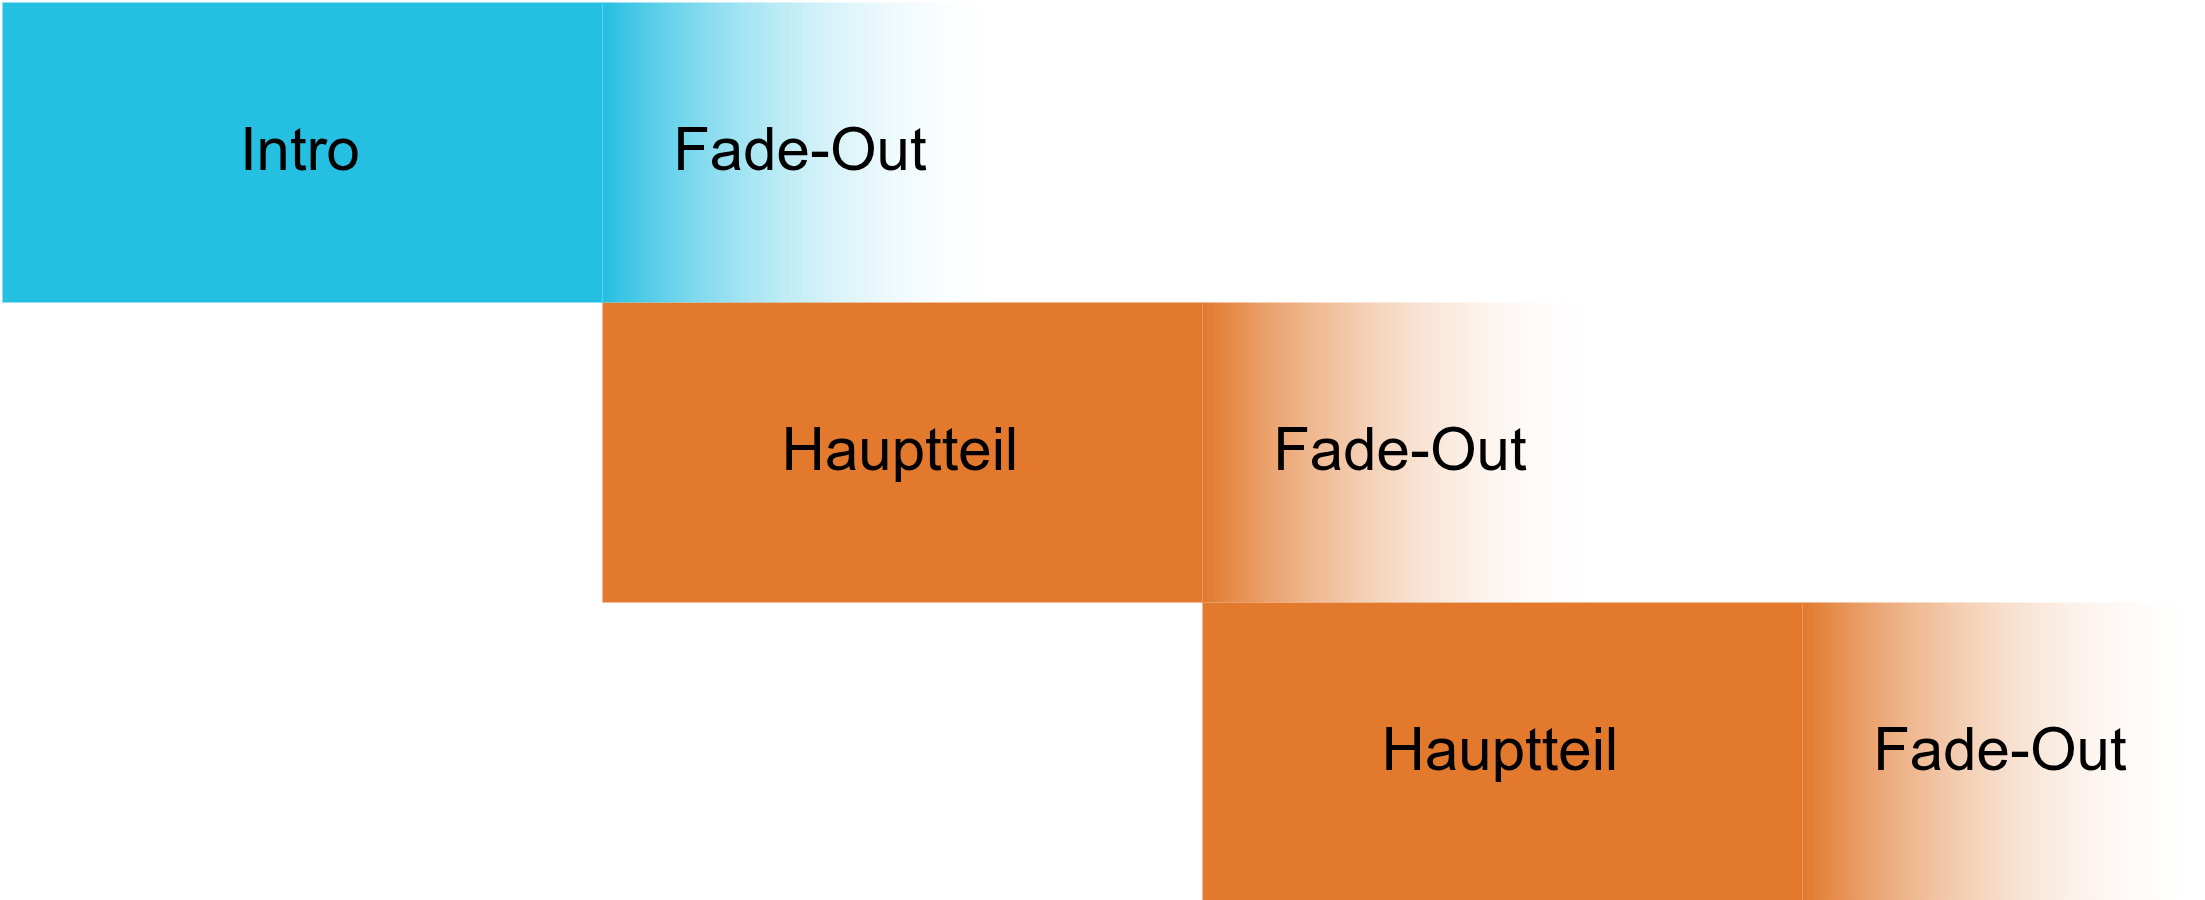
\includegraphics[width=0.8\linewidth]{bilder/Songstruktur.drawio.png}
	\caption{Kompositionsstruktur}
	\label{programm:engine:sound:übergang:bild}
\end{figure}

Die Teile des Stückes lassen sich nicht linear
hintereinander abspielen, da sie jeweils ausklingen,
während der nächste Teil bereits spielt. Es müssen
also mehrere Teile parallel spielen.

Um dieses Problem zu Lösen, bietet die Engine ein Besonderes
Objekt: \texttt{MusicLoopObject} aus dem Paket \texttt{czg.objects.music\_loop\_object}.
Von diesem darf es genau eines pro Szene geben. Ist es
vorhanden, spielt es seine eingespeicherten Segmente
so ab, dass diese, wie in \ref{programm:engine:sound:übergang:bild}
dargestellt, ineinander übergehen.

Die Klasse selbst speichert zwei als \texttt{private static final}
deklarierte Werte:

\begin{itemize}
	\item Einen eigenen \textit{Wiedergabethread}
	\item Eine \texttt{java.util.concurrent.atomic.AtomicReference}, die
	      die Instanz von \texttt{MusicLoopObject} speichert und sonst
	      \texttt{null} ist.
\end{itemize}

Instanzen der Klasse beinhalten zwei weitere Daten:

\begin{itemize}
	\item Eine \texttt{Map<BaseSound, SegmentChangeMarker>}, welche die
	      Segmente des Stücks speichert. \texttt{SegmentChangeMarker}
	      wird in kürze näher erläutert.
	\item Den \texttt{BaseSound}, welcher das aktuell abgespielte
	      Segment darstellt.
\end{itemize}

Der Konstruktor der Klasse nimmt keine Parameter und delegiert
zu dem der Elternklasse \texttt{BaseObject}: Das Objekt hat kein
Bild, eine Größe von $0 \times 0$ Pixeln und ist an der willkürlich
gewählten Position $(0|0)$ platziert. Die \texttt{draw}-Methode
wird zusätzlich noch überschrieben und mit einem leeren Körper
versehen.

Die eigentliche Konfiguration von \texttt{MusicLoopObject} findet
über dessen \texttt{addSegment(BaseSound, SegmentChangeMarker)}
statt. Dabei ist \texttt{SegmentChangeMarker} eine \texttt{record}-Klasse,
welche lediglich zwei Daten speichert:

\begin{enumerate}
	\item Die Wiedergabeposition in Millisekunden, an welcher das
	      nächste Wiedergabesegment spielen soll.
	\item Das nächste Segment in Form eines \texttt{BaseSound}.
\end{enumerate}

\texttt{addSegment} prüft nun zunächst, ob bereits ein Sound als
aktuelles Segment gespeichert ist. Wenn nicht, übernimmt der
übergebene Sound diese Rolle. Dieser wird dann außerdem dem
angegebenen \texttt{SegmentChangeMarker} in der \texttt{Map}
mit den Segmenten zugeordnet.

Um nun die Wiedergabe des Stücks zu beginnen, muss die Methode
\texttt{MusicLoopObject.start} aufgerufen werden. Diese prüft
zunächst, dass sich bisher keine andere Instanz der Klasse in
die \texttt{AtomicReference} eingespeichert hat. Ist dies nicht
der Fall, wird das aktuelle \texttt{MusicLoopObject} dort hinterlegt.
Dann wird das erste Segment mit \texttt{BaseSound.setPlaying}
gestartet. Der Wiedergabethread wird ggf. gestartet und mit der
\texttt{notify}-Methode bei Bedarf geweckt.

Beim Aufruf von \texttt{BaseObject.unload} über \texttt{MusicLoopObject}
wird der Wiedergabethread mit \texttt{Thread.interrupt} unterbrochen
und die \texttt{AtomicReference} wird wieder auf \texttt{null}
gesetzt.
\\

Der Wiedergabethread führt die private, statische Methode
\texttt{MusicLoopObject.segmentChangeThreadLoop}. Diese
besteht aus einer Endlosschleife, welche zwei wesentliche
Schritte wiederholt:

\begin{enumerate}
	\item Solange die in der \texttt{AtomicReference} hinterlegte
	      Instanz nicht \texttt{null} ist, wird gewartet, bis das
	      nächste Segment abgespielt werden sollte, woraufhin dies
	      auch getan wird:
	      \begin{enumerate}
	      	\item Der Thread wird für die im \texttt{SegmentChangeMarker}
	      	      angegebene Zeit mit \texttt{Thread.sleep} pausiert.
	      	\item Das aktuelle Segment der \texttt{MusicLoopObject}-Instanz
	      	      wird auf den im \texttt{SegmentChangeMarker} hinterlegten
	      	      \texttt{BaseSound} gesetzt.
	      	\item Letzterer wird mit \texttt{BaseSound.setPlaying} gestartet.
	      \end{enumerate}
	\item Warten auf das Aufwecken des Threads über den Aufruf
	      des Konstruktors der Klasse.
\end{enumerate}


\subsection{Hilfsklassen}

Zuletzt enthält die Engine noch einige staatische Hilfsmethoden und
Konstanten , welche auf entsprechende Klassen aufgeteilt sind.

\subsubsection{\texttt{czg.util.Draw}}

Diese Klasse enthält \texttt{java.awt.Font}-Objekte, um einheitlich zu
verwendende Schriftarten bereitzustellen, sowie eine Methode, welche
eine beliebige Zeichenkette mithilfe eines gegebenen Grafikkontexts unter
Angabe des Mittelpunkts des Schriftzugs zeichnet.


\subsubsection{\texttt{czg.util.Images}}

Diese Klasse wird verwendet, um Bilder aus Dateien in den Speicher zu
laden sowie diese zu drehen.

\paragraph{Die \texttt{get(String)}-Methode} versucht, ein Bild von
dem angegebenen Dateipfad zu laden. Gelingt dies nicht, gibt sie ein
Platzhalterbild zurück. Ist letzteres im Spiel zu sehen, ist dies ein
klares Signal, dass es einen Fehler beim Laden eines Bildes gab.

\begin{figure}[H]
	\centering
	
\includegraphics[width=0.15\linewidth]{bilder/fallback_textur.png}
	\caption{Platzhalterbild}
	\label{programm:engine:fallback-textur}
\end{figure}

\texttt{get} verwendet eine \texttt{HashMap}, in welcher bei ihrem
Aufruf der Dateipfad dem geladenen Bild zugeordnet wird. So bleiben
geladene Bilder im Speicher und müssen nicht oft erneut geladen werden.

\paragraph{\texttt{rotateImage(Image, double)}} dreht das gegebene Bild
um den gegebenen Winkel in mathematisch negative Richtung, also im
Uhrzeigersinn. Dafür werden die Klassen \texttt{AffineTransform}
sowie \texttt{AffineTransformOp} aus dem Paket \texttt{java.awt.geom}
verwendet. Zusätzlich werden völlig transparente Teile des gedrehten
Bildes von den Rändern her abgeschnitten.


\subsection{czg.util.Sounds}

Diese Klasse definiert ein \texttt{javax.sound.sampled.AudioFormat}, welches
in der Engine zu verwenden ist, sowie eine \texttt{getInputStream(String)}-Methode,
welche einen \texttt{AudioInputStream} für die gegebene Datei in dem eben genannten
Format erstellt.


\end{sloppypar}